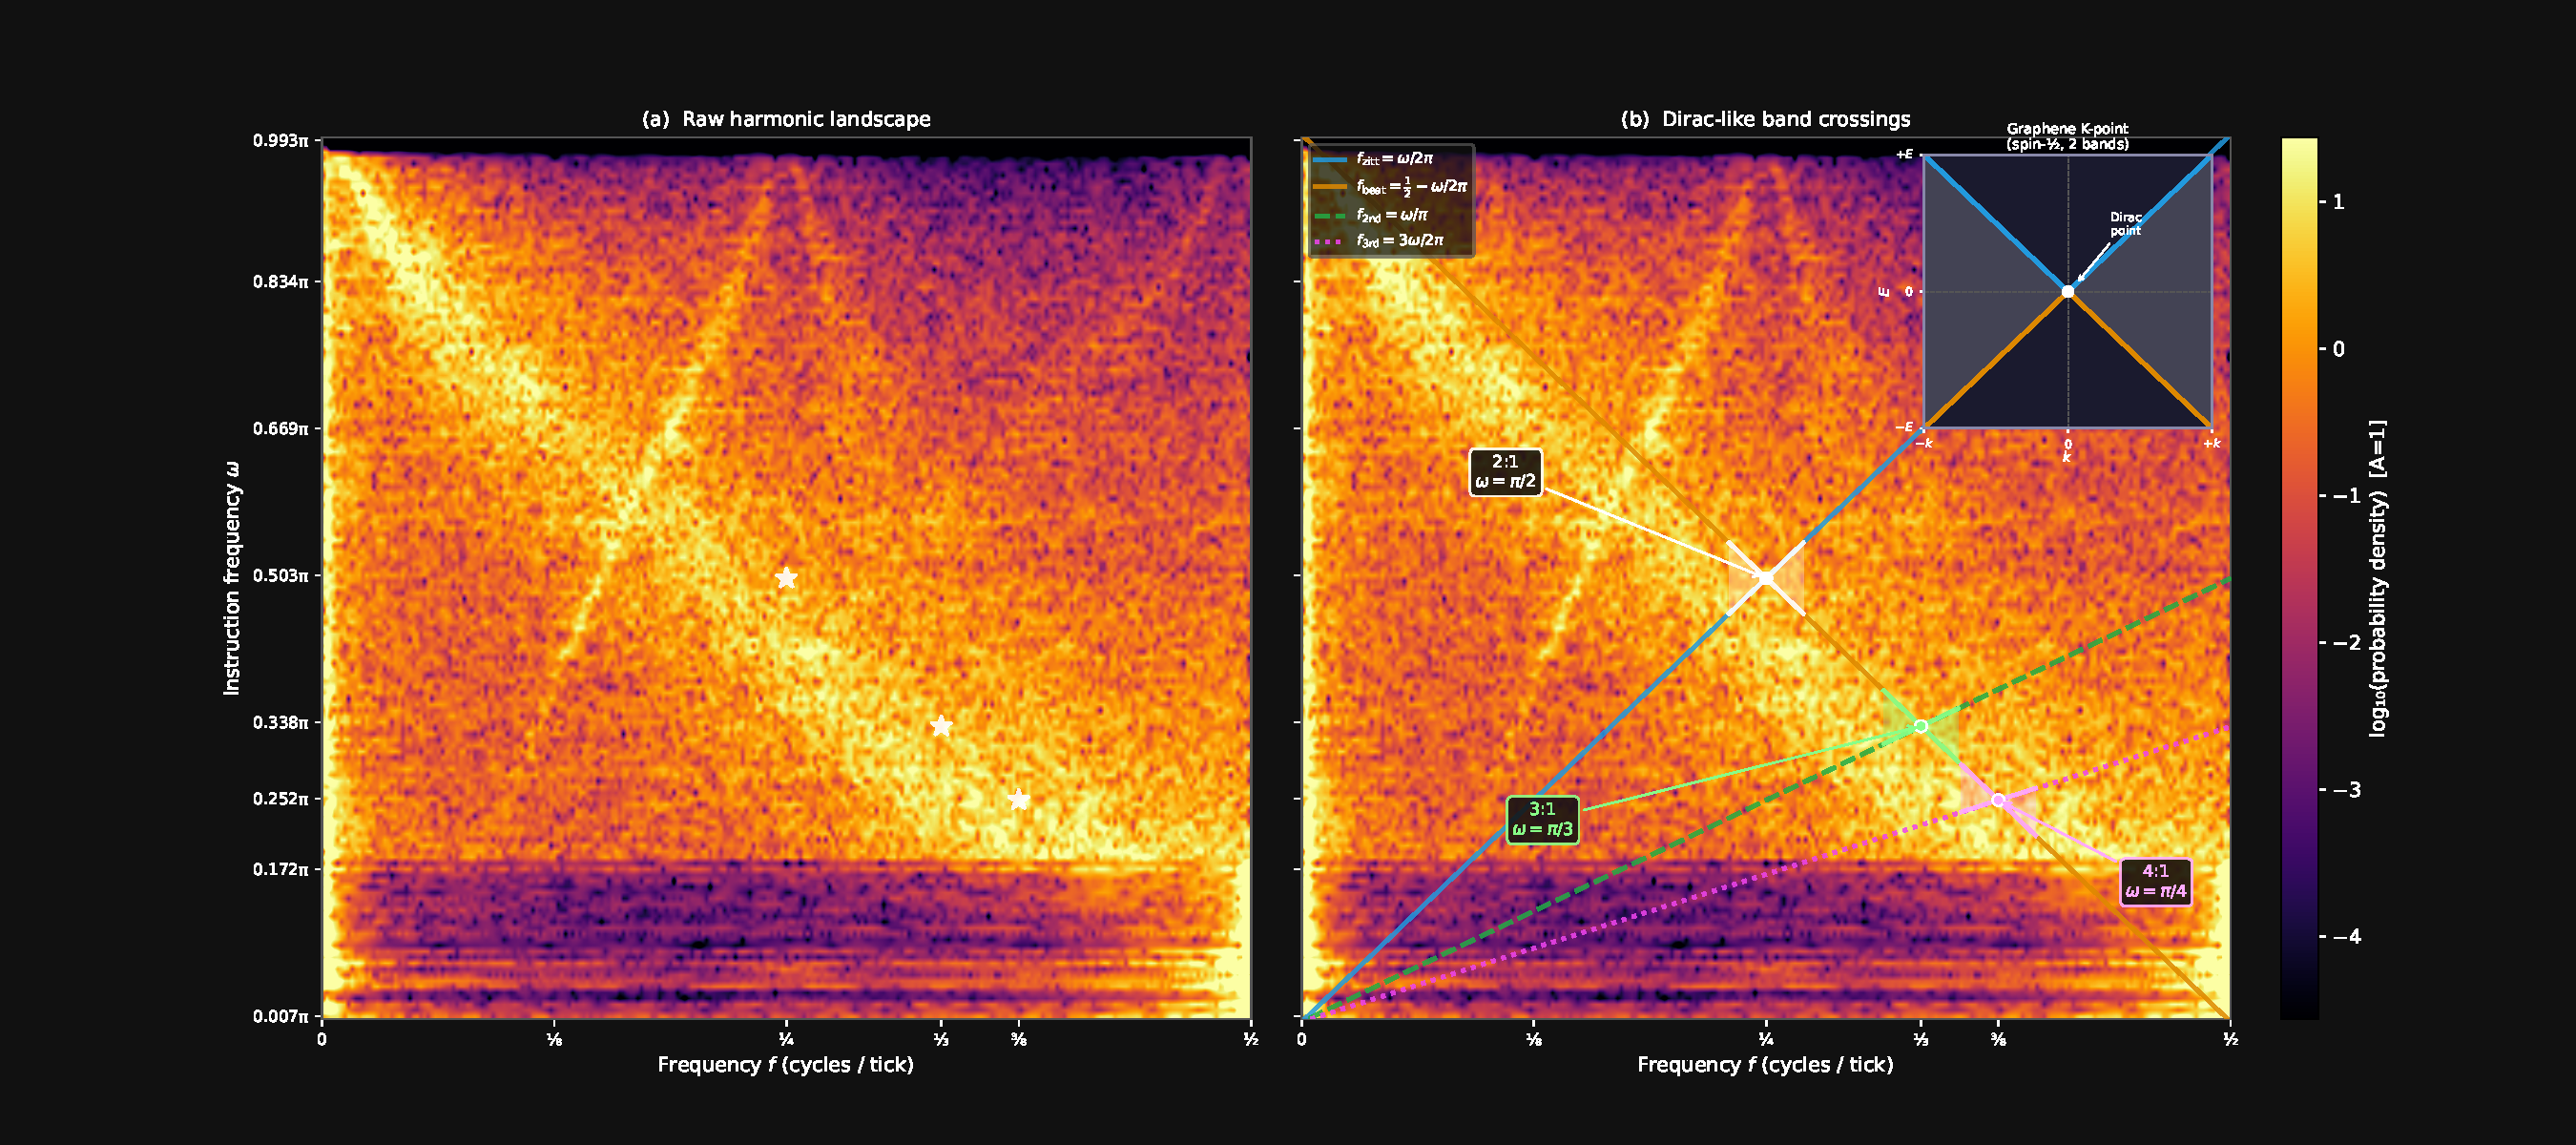
\includegraphics[width=\textwidth]{../figures/dirac_cones_doublepane}
\label{fig:dirac_cones}
\caption{Dirac-like band crossings in the harmonic fingerprint of the
$T^3_\text{diamond}$ lattice.
\textbf{Both panels:} colour encodes the spectral power of the
\texttt{rgb\_cmy\_imbalance} signal --- the difference
$|\psi_R|^2 - |\psi_L|^2$ summed over the lattice --- for 150 free
particles scanned over instruction frequency $\omega \in (0,\pi)$
(vertical axis, lattice mass proxy).
Warmth is probability density --- the $A=1$ constraint made visible.
A bright region at $(\omega, f)$ means that a particle of mass $\omega$
has its probability density oscillating coherently between the RGB and
CMY sublattices at frequency $f$; the total probability is conserved
($A=1$) at every tick, so the spectral structure encodes how probability
is redistributed, never created or destroyed.
Dark regions carry no coherent probability current at those frequencies.
%
\textbf{(a) Raw landscape.}
Three zones emerge without annotation.
\emph{Bottom band} ($\omega \to 0$, metallic limit): a near-massless
particle has $p_\text{stay} \approx 0$ and flows freely across both
sublattices; its probability density oscillates at all frequencies
simultaneously, saturating the spectrum.
\emph{Two diagonal bands}: the Zitterbewegung fundamental
$f_\text{zitt} = \omega/2\pi$ (rising) and its vacuum beat
$f_\text{beat} = \tfrac{1}{2} - \omega/2\pi$ (falling) are the
dominant modes of chiral probability oscillation.
Their widths in $\omega$ are the Arnold tongue locking basins, in which
probability redistribution locks to a rational fraction of the vacuum
tick rate; width decreases with resonance order by the Farey hierarchy.
\emph{Dark upper-left triangle} (insulating limit): a heavy particle
($\omega \to \pi$, $p_\text{stay} \to 1$) barely hops; probability
density is nearly frozen and only oscillates at $f_\text{zitt}$ and
$f_\text{beat}$, leaving the rest of the spectrum silent.
White stars mark the three principal resonance lock-in points.
%
\textbf{(b) Annotated crossings.}
Overlaid theory lines identify three Dirac-like crossings where the
probability density simultaneously resonates in two harmonic modes ---
precisely the condition for Arnold tongue lock-in and hence stable
particle formation:
\begin{itemize}[noitemsep,topsep=2pt]
  \item \textbf{2:1} at $(\omega, f) = (\pi/2,\,\tfrac{1}{4})$:
        $f_\text{zitt} \cap f_\text{beat}$, symmetric slopes $\pm 2\pi$,
        widest tongue.  The physical proton mass sits at the centre of
        this tongue, maximising orbital stability.
  \item \textbf{3:1} at $(\pi/3,\,\tfrac{1}{3})$:
        $f_\text{2nd} \cap f_\text{beat}$, asymmetric slopes ($\pi$
        vs.\ $-2\pi$).  The hydrogen ground state satisfies
        $\omega_e R_1 = \pi/3$ to $0.23\%$, locking atomic probability
        density to this crossing.
  \item \textbf{4:1} at $(\pi/4,\,\tfrac{3}{8})$:
        $f_\text{3rd} \cap f_\text{beat}$, slopes $\tfrac{2\pi}{3}$
        vs.\ $-2\pi$; most asymmetric crossing, narrowest tongue.
\end{itemize}
Each crossing is a linear touching of two probability-oscillation modes
in $(\omega, f)$ space, directly analogous to the Dirac point at
graphene's K-point (inset: standard $(k,E)$ picture, spin-$\tfrac{1}{2}$,
two symmetric bands).
Unlike graphene's symmetric $\pm v_F k$ cone, the 3:1 and 4:1 crossings
are intrinsically asymmetric --- a zero-free-parameter consequence of the
bipartite lattice geometry.
Probability density is the primary observable throughout: quantisation,
the Bohr spectrum, and the Standard Model particle zoo are all
consequences of which rational frequency ratios admit stable, coherent
chiral probability oscillation on the $T^3_\text{diamond}$ lattice.}
